\documentclass[margin=.2cm]{standalone}

\usepackage{tikz}
\usetikzlibrary{calc,arrows,positioning}

\pgfdeclarelayer{bg}    % declare background layer
\pgfsetlayers{bg,main}  % set the order of the layers (main is the standard layer)


\begin{document}

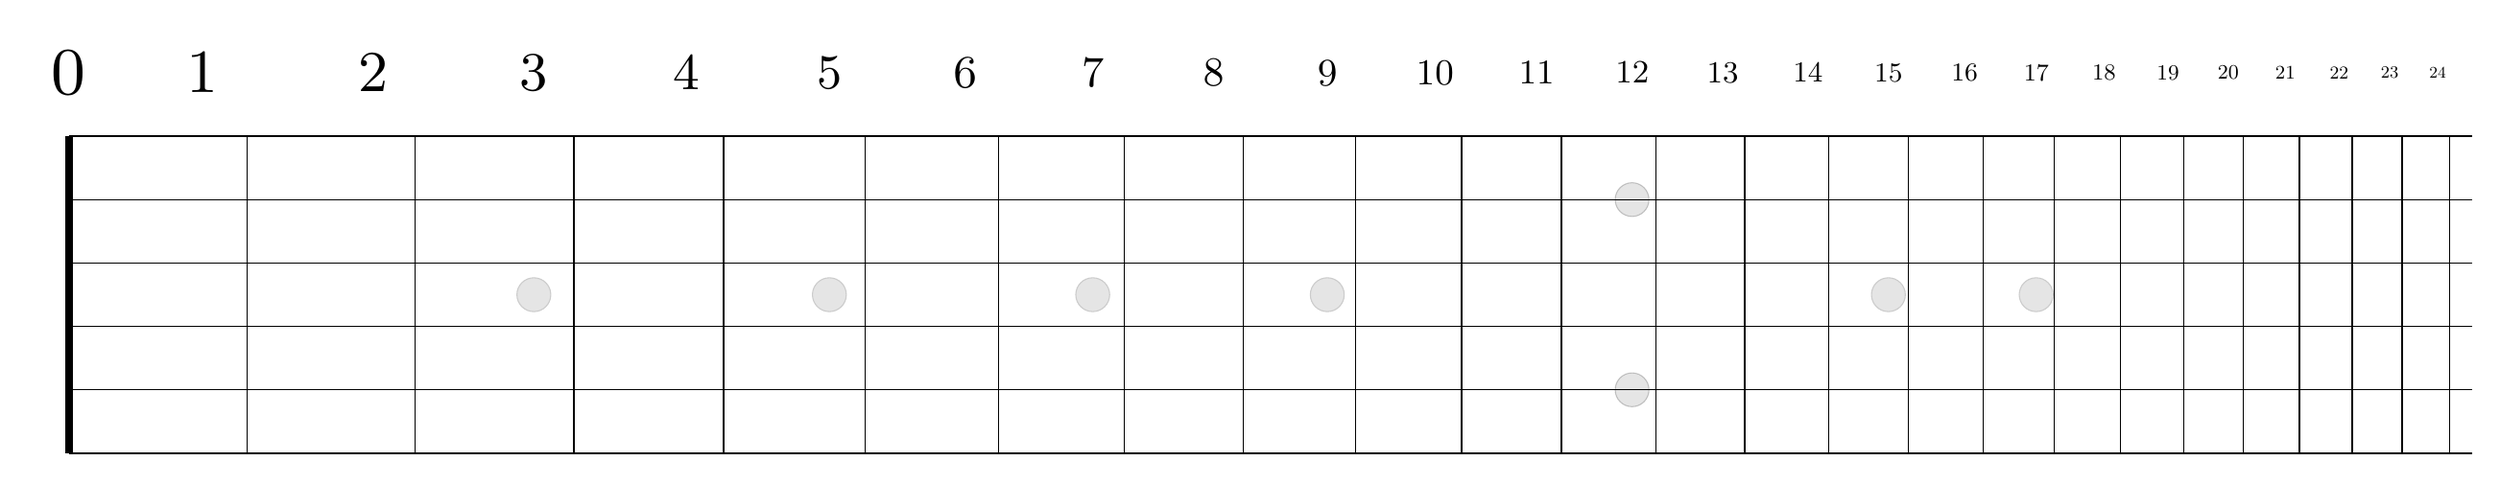
\begin{tikzpicture}[
    ynode/.style={draw=red!50,circle,fill=red!50,scale=.35,inner sep=1pt,minimum size=1.7em}, thick,scale=2.8, every node/.style={scale=2.8}]

  \def\basestrings{{4, 9, 2, 7, 0, 5}}
   
  \def\fretscaleratio{0.94387431268} % 1/2^(1/12)
  %%%% Draw the base and set coordinates %%%%
  %% x direction goes in opposite way
  \begin{scope}[xscale=-15,yscale=.3,line width=.5]
  

    \xdef\x{1}

    %% Left line
    \draw[line width=3] (1,1) -- (1,6);
    \foreach \fret in {1,...,24}{
    
        % x starts at 1 and we keep multiplying by a number in range (0, 1) 
        % x -------------------------> 0
        % x -----|-------------------> 0
        %   {   }{___________________}
        %     |            |
        %     |    n = x * 1/(2^(1/12)))   
        %   m = x - n  
        % therefore
        % x ---|-|-------------------> 0
        %      |
        %      |
        %    m/4  + n = text-position  
        \pgfmathsetmacro\textpos{ (\x -  \x * \fretscaleratio)/4 + (\x * \fretscaleratio)}
        
          %% Set coordinate for each string
          \foreach \str in {1,...,6}{
            \coordinate (\fret-\str) at (\textpos,\str);
            \pgfmathsetmacro\cap{int(mod(\basestrings[\str - 1] + \fret, 12))}
            % Draw the number on each fret position
            % \node [scale=0.97193715634*\x] at (\fret-\str) {\cap};
          }
          %% Set coordinate for the text above
          \pgfmathsetmacro\x{\x * \fretscaleratio} % re-scale the string based on last fret
          \xdef\x{\x}
          %% Draw the fret
          \draw (\x,1) -- (\x,6);
          
        \node [scale=0.97193715634*\x] at (\textpos, 7) {\small \fret};
    }

    %% Draw strings
    \foreach \str in {1,...,6}{
      \draw (1,\str) -- (0.97153194115*\x,\str);
      \coordinate (start\str) at (1,\str); % define nut area
    }
    \coordinate (nut) at (1,7);
   
  \end{scope}

  %% Draw fret circle marks
  \begin{pgfonlayer}{bg}    % select the background layer
      \foreach \f in {3,5,7,9,15,17}{
        \draw[black!20,fill=black!10] ($(\f-3)!.5!(\f-4)$) circle (.08);
      }
      
      \draw[opacity=.20,fill,fill opacity=.10] (12-2) circle (.08) (12-5) circle (.08);
  \end{pgfonlayer}
  
  % define the open string
  \newcommand\savename[2]{\expandafter\xdef\csname name#1\endcsname{#2}}
  \newcommand\getname[1]{\csname name#1\endcsname}
  \foreach \n/\t in {1/$9$,2/10,3/$11$,4/0,5/1,6/$2$,7/3,8/$4$,9/5,10/6,11/$7$,0/8}{
    \savename{\n}{\t}
  }
  % draw the open string numbers
%   \foreach [count=\str] \strnote in {9, 2, 7, 0, 5, 10} {
%     \node[anchor=east] at (start\str) {\strnote};
%   }

\node[scale=1] at (nut) {\small 0}; % add zero-th fret


\end{tikzpicture}

\end{document}
